\documentclass[10pt,oneside]{article}
\usepackage[T1]{fontenc}
\usepackage[utf8]{inputenc}
%\usepackage[latin1]{inputenc}
\DeclareUnicodeCharacter{00A0}{ }
% \usepackage{lmodern}
%\usepackage[adobe-utopia,uppercase=upright,greeklowercase=upright]{mathdesign}
\usepackage[adobe-utopia]{mathdesign}
%\usepackage{minionpro}
% \usepackage{pifont}
% \usepackage{amssymb}
\usepackage{amsmath}
\usepackage[francais]{babel}
% \usepackage[francais]{varioref}
\usepackage[dvips]{graphicx}
\usepackage{here}
\usepackage{framed}
\usepackage[normalem]{ulem}
\usepackage{fancyhdr}
\usepackage{titlesec}
\usepackage{vmargin}
\usepackage{longtable}

\usepackage{amsmath}

\usepackage{ifthen}
%\usepackage[•]{caption}

%\usepackage{epsfig}
\usepackage{subfig}

\usepackage{multirow}
\usepackage{multicol} % Portions de texte en colonnes
\usepackage{flafter}%floatants après la référence



\usepackage{color}
\usepackage{colortbl}


\definecolor{gris25}{gray}{0.75}
\definecolor{bleu}{RGB}{18,33,98}
\definecolor{bleuf}{RGB}{42,94,171}
\definecolor{bleuc}{RGB}{231,239,247}
\definecolor{rougef}{RGB}{185,18,27}
\definecolor{rougec}{RGB}{255,230,231}
\definecolor{vertf}{RGB}{103,126,82}
\definecolor{vertc}{RGB}{220,255,191}
\definecolor{violetf}{RGB}{112,48,160}
\definecolor{violetc}{RGB}{230,224,236}
\definecolor{jaunec}{RGB}{220,255,191}

\newenvironment{sci}[1][\hsize]%
{%
    \def\FrameCommand%
    {%
%\rotatebox{90}{\textit{\textsf{Scilab}}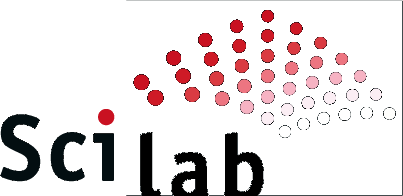
\includegraphics[height=.8cm]{png/logo_scilab}} 
\rotatebox{90}{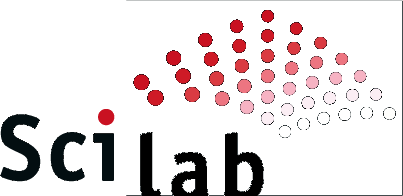
\includegraphics[height=.6cm]{png/logo_scilab}} 
        {\color{violetf}\vrule width 3pt}%
        \hspace{0pt}%must no space.
        \fboxsep=\FrameSep\colorbox{violetc}%
    }%
    \MakeFramed{\hsize #1 \advance\hsize-\width\FrameRestore}%
}%
{\endMakeFramed}%

\newenvironment{pseudo}[1][\hsize]%
{%
    \def\FrameCommand%
    {%
\rotatebox{90}{\textit{\textsf{Pseudo Code}}} 
        {\color{violetf}\vrule width 3pt}%
        \hspace{0pt}%must no space.
        \fboxsep=\FrameSep\colorbox{violetc}%
    }%
    \MakeFramed{\hsize #1 \advance\hsize-\width\FrameRestore}%
}%
{\endMakeFramed}%

\newenvironment{py}[1][\hsize]%
{%
    \def\FrameCommand%
    {%
%\rotatebox{90}{\textit{\textsf{Python}}} 
\rotatebox{90}{
\includegraphics[height=.6cm]{png/logo_python}} 
        {\color{violetf}\vrule width 3pt}%
        \hspace{0pt}%must no space.
        \fboxsep=\FrameSep\colorbox{violetc}%
    }%
    \MakeFramed{\hsize #1 \advance\hsize-\width\FrameRestore}%
}%
{\endMakeFramed}%


\newenvironment{term}[1][\hsize]%
{%
    \def\FrameCommand%
    {%
\rotatebox{90}{\textit{\textsf{Terminal}}} 
        {\color{violetf}\vrule width 3pt}%
        \hspace{0pt}%must no space.
        \fboxsep=\FrameSep\colorbox{violetc}%
    }%
    \MakeFramed{\hsize #1 \advance\hsize-\width\FrameRestore}%
}%
{\endMakeFramed}%


\newenvironment{rem}[1][\hsize]%
{%
    \def\FrameCommand
    {%
\rotatebox{90}{\textit{\textsf{Remarque}}} 
        {\color{bleuf}\vrule width 3pt}%
        \hspace{0pt}%must no space.
        \fboxsep=\FrameSep\colorbox{bleuc}%
    }%
    \MakeFramed{\hsize#1\advance\hsize-\width\FrameRestore}%
}%
{\endMakeFramed}%


\newenvironment{savoir}[1][\hsize]%
{%
    \def\FrameCommand
    {%
\rotatebox{90}{\textit{\textsf{Savoir}}} 
        {\color{bleuf}\vrule width 3pt}%
        \hspace{0pt}%must no space.
        \fboxsep=\FrameSep\colorbox{bleuc}%
    }%
    \MakeFramed{\hsize#1\advance\hsize-\width\FrameRestore}%
}%
{\endMakeFramed}%

\newenvironment{objectif}[1][\hsize]%
{%
    \def\FrameCommand
    {%
\rotatebox{90}{\textit{\textsf{Objectif}}} 
        {\color{rougef}\vrule width 3pt}%
        \hspace{0pt}%must no space.
        \fboxsep=\FrameSep\colorbox{rougec}%
    }%
    \MakeFramed{\hsize#1\advance\hsize-\width\FrameRestore}%
}%
{\endMakeFramed}%

\newenvironment{prob}[1][\hsize]%
{%
    \def\FrameCommand%
    {%
\rotatebox{90}{\textit{\textsf{ Problématique}}} 
        {\color{rougef}\vrule width 3pt}%
        \hspace{0pt}%must no space.
        \fboxsep=\FrameSep\colorbox{rougec}%
    }%
    \MakeFramed{\hsize#1\advance\hsize-\width\FrameRestore}%
}%
{\endMakeFramed}%

\newenvironment{obj}[1][\hsize]%
{%
    \def\FrameCommand%
    {%
\rotatebox{90}{\textit{\textsf{ $\;$}}} 
        {\color{rougef}\vrule width 3pt}%
        \hspace{0pt}%must no space.
        \fboxsep=\FrameSep\colorbox{rougec}%
    }%
    \MakeFramed{\hsize#1\advance\hsize-\width\FrameRestore}%
}%
{\endMakeFramed}%

\newenvironment{defi}[1][\hsize]%
{%
    \def\FrameCommand%
    {%
\rotatebox{90}{\textit{\textsf{Définition\\}}} 
        {\color{bleuf}\vrule width 3pt}%
        \hspace{0pt}%must no space.
        \fboxsep=\FrameSep\colorbox{bleuc}%
    }%
    \MakeFramed{\hsize#1\advance\hsize-\width\FrameRestore}%
}%
{\endMakeFramed}%


\newenvironment{demo}[1][\hsize]%
{%
    \def\FrameCommand%
    {%
\rotatebox{90}{\textit{\textsf{Démonstration\\}}} 
        {\color{bleuf}\vrule width 3pt}%
        \hspace{0pt}%must no space.
        \fboxsep=\FrameSep\colorbox{bleuc}%
    }%
    \MakeFramed{\hsize#1\advance\hsize-\width\FrameRestore}%
}%
{\endMakeFramed}%


\newenvironment{hypo}[1][\hsize]%
{%
    \def\FrameCommand%
    {%
\rotatebox{90}{\textit{\textsf{Hypothèse\\}}} 
        {\color{bleuf}\vrule width 3pt}%
        \hspace{0pt}%must no space.
        \fboxsep=\FrameSep\colorbox{bleuc}%
    }%
    \MakeFramed{\hsize#1\advance\hsize-\width\FrameRestore}%
}%
{\endMakeFramed}%


\newenvironment{prop}[1][\hsize]%
{%
    \def\FrameCommand%
    {%
\rotatebox{90}{\textit{\textsf{Propriété\\}}} 
        {\color{bleuf}\vrule width 3pt}%
        \hspace{0pt}%must no space.
        \fboxsep=\FrameSep\colorbox{bleuc}%
    }%
    \MakeFramed{\hsize#1\advance\hsize-\width\FrameRestore}%
}%
{\endMakeFramed}%

\newenvironment{props}[1][\hsize]%
{%
    \def\FrameCommand%
    {%
\rotatebox{90}{\textit{\textsf{Propriétés\\}}} 
        {\color{bleuf}\vrule width 3pt}%
        \hspace{0pt}%must no space.
        \fboxsep=\FrameSep\colorbox{bleuc}%
    }%
    \MakeFramed{\hsize#1\advance\hsize-\width\FrameRestore}%
}%
{\endMakeFramed}%

\newenvironment{exemple}[1][\hsize]%
{%
    \def\FrameCommand%
    {%
\rotatebox{90}{\textit{\textsf{Exemple\\}}} 
        {\color{vertf}\vrule width 3pt}%
        \hspace{0pt}%must no space.
        \fboxsep=\FrameSep\colorbox{vertc}%
    }%
    \MakeFramed{\hsize#1\advance\hsize-\width\FrameRestore}%
}%
{\endMakeFramed}%

\newenvironment{exercice}[1][\hsize]%
{%
    \def\FrameCommand%
    {%
\rotatebox{90}{\textit{\textsf{Exercice\\}}} 
        {\color{vertf}\vrule width 3pt}%
        \hspace{0pt}%must no space.
        \fboxsep=\FrameSep\colorbox{vertc}%
    }%
    \MakeFramed{\hsize#1\advance\hsize-\width\FrameRestore}%
}%
{\endMakeFramed}%

\newenvironment{Support}[1][\hsize]%
{%
    \def\FrameCommand%
    {%
\rotatebox{90}{\textit{\textsf{Support de cours\\}}} 
        {\color{vertf}\vrule width 3pt}%
        \hspace{0pt}%must no space.
        \fboxsep=\FrameSep\colorbox{jaunec}%
    }%
    \MakeFramed{\hsize#1\advance\hsize-\width\FrameRestore}%
}%
{\endMakeFramed}%

\newenvironment{resultat}[1][\hsize]%
{%
    \def\FrameCommand%
    {%
\rotatebox{90}{\textit{\textsf{Résultat\\}}} 
        {\color{rougef}\vrule width 3pt}%
        \hspace{0pt}%must no space.
        \fboxsep=\FrameSep\colorbox{rougec}%
    }%
    \MakeFramed{\hsize#1\advance\hsize-\width\FrameRestore}%
}%
{\endMakeFramed}%

\newenvironment{methode}[1][\hsize]%
{%
    \def\FrameCommand%
    {%
\rotatebox{90}{\textit{\textsf{Méthode\\}}} 
        {\color{rougef}\vrule width 3pt}%
        \hspace{0pt}%must no space.
        \fboxsep=\FrameSep\colorbox{rougec}%
    }%
    \MakeFramed{\hsize#1\advance\hsize-\width\FrameRestore}%
}%
{\endMakeFramed}%

\newenvironment{theo}[1][\hsize]%
{%
    \def\FrameCommand%
    {%
\rotatebox{90}{\textit{\textsf{Théorème\\}}} 
        {\color{rougef}\vrule width 3pt}%
        \hspace{0pt}%must no space.
        \fboxsep=\FrameSep\colorbox{rougec}%
    }%
    \MakeFramed{\hsize#1\advance\hsize-\width\FrameRestore}%
}%
{\endMakeFramed}%

\newenvironment{warn}[1][\hsize]%
{%
    \def\FrameCommand%
    {%
\rotatebox{90}{\textit{\textsf{Attention\\}}} 
        {\color{rougef}\vrule width 3pt}%
        \hspace{0pt}%must no space.
        \fboxsep=\FrameSep\colorbox{rougec}%
    }%
    \MakeFramed{\hsize#1\advance\hsize-\width\FrameRestore}%
}%
{\endMakeFramed}%

% \usepackage{pstricks}
%\usepackage{minitoc}
% \setcounter{minitocdepth}{4}

\setcounter{tocdepth}{2}

% \mtcselectlanguage{french} 

%\usepackage{draftcopy}% "Brouillon"
% \usepackage{floatflt}
\usepackage{psfrag}
%\usepackage{listings} % Permet d'insérer du code de programmation
\renewcommand{\baselinestretch}{1.2}

% Changer la numérotation des figures :
% ------------------------------------
% \makeatletter
% \renewcommand{\thefigure}{\ifnum \c@section>\z@ \thesection.\fi
%  \@arabic\c@figure}
% \@addtoreset{figure}{section}
% \makeatother
 


%%%%%%%%%%%%
% Définition des vecteurs %
%%%%%%%%%%%%
 \newcommand{\vect}[1]{\overrightarrow{#1}}

%%%%%%%%%%%%
% Définition des torseusr %
%%%%%%%%%%%%

 \newcommand{\torseur}[1]{%
\left\{{#1}\right\}
}

\newcommand{\torseurcin}[3]{%
\left\{\mathcal{#1} \left(#2/#3 \right) \right\}
}

\newcommand{\torseurstat}[3]{%
\left\{\mathcal{#1} \left(#2\rightarrow #3 \right) \right\}
}

 \newcommand{\torseurc}[8]{%
%\left\{#1 \right\}=
\left\{
{#1}
\right\}
 = 
\left\{%
\begin{array}{cc}%
{#2} & {#5}\\%
{#3} & {#6}\\%
{#4} & {#7}\\%
\end{array}%
\right\}_{#8}%
}

 \newcommand{\torseurcol}[7]{
\left\{%
\begin{array}{cc}%
{#1} & {#4}\\%
{#2} & {#5}\\%
{#3} & {#6}\\%
\end{array}%
\right\}_{#7}%
}

 \newcommand{\torseurl}[3]{%
%\left\{\mathcal{#1}\right\}_{#2}=%
\left\{%
\begin{array}{l}%
{#1} \\%
{#2} %
\end{array}%
\right\}_{#3}%
}

 \newcommand{\vectv}[3]{%
\vect{V\left( {#1} \in {#2}/{#3}\right)}
}


\newcommand{\vectf}[2]{%
\vect{R\left( {#1} \rightarrow {#2}\right)}
}

\newcommand{\vectm}[3]{%
\vect{\mathcal{M}\left( {#1}, {#2} \rightarrow {#3}\right)}
}


 \newcommand{\vectg}[3]{%
\vect{\Gamma \left( {#1} \in {#2}/{#3}\right)}
}

 \newcommand{\vecto}[2]{%
\vect{\Omega\left( {#1}/{#2}\right)}
}
% }$$\left\{\mathcal{#1} \right\}_{#2} =%
% \left\{%
% \begin{array}{c}%
%  #3 \\%
%  #4 %
% \end{array}%
% \right\}_{#5}}

%  ------------------------------------------
% | Modification du formatage des sections : | 
%  ------------------------------------------

% Grands titres :
% ---------------

\newcommand{\titre}[1]{%
\begin{center}
      \bigskip
      \rule{\textwidth}{1pt}
      \par\vspace{0.1cm}
      
      \textbf{\large #1}
      \par\rule{\textwidth}{1pt}
    \end{center}
    \bigskip
  }

% Supprime le numéro du chapitre dans la numérotation des sections:
% -----------------------------------------------------------------
\makeatletter
\renewcommand{\thesection}{\@arabic\c@section}
\makeatother


% \titleformat{\chapter}[display]
% {\normalfont\Large\filcenter}
% {}
% {1pc}
% {\titlerule[1pt]
%   \vspace{1pc}%
%   \Huge}[\vspace{1ex}%
% \titlerule]


%%%% Chapitres Comme PY Pechard %%%%%%%%%
% numéro du chapitre
\DeclareFixedFont{\chapnumfont}{OT1}{phv}{b}{n}{80pt}
% pour le mot « Chapitre »
\DeclareFixedFont{\chapchapfont}{OT1}{phv}{m}{it}{40pt}
% pour le titre
\DeclareFixedFont{\chaptitfont}{T1}{phv}{b}{n}{25pt}

\definecolor{gris}{gray}{0.75}
\titleformat{\chapter}[display]%
	{\sffamily}%
	{\filleft\chapchapfont\color{gris}\chaptertitlename\
	\\
	\vspace{12pt}
	\chapnumfont\thechapter}%
	{16pt}%
	{\filleft\chaptitfont}%
	[\vspace{6pt}\titlerule\titlerule\titlerule]

%%%%  Fin Chapitres Comme PY Pechard %%%%%%%%%


% Section, subsection, subsubsection sans serifs :
% % ----------------------------------------------

% \makeatletter
% \renewcommand{\section}{\@startsection{section}{0}{0mm}%
% {\baselineskip}{.3\baselineskip}%
% {\normalfont\sffamily\Large\textbf}}%
% \makeatother

\makeatletter
\renewcommand{\@seccntformat}[1]{{\textcolor{bleu}{\csname
the#1\endcsname}\hspace{0.5em}}}
\makeatother

\makeatletter
\renewcommand{\section}{\@startsection{section}{1}{\z@}%
                       {-4ex \@plus -1ex \@minus -.4ex}%
                       {1ex \@plus.2ex }%
                       {\normalfont\Large\sffamily\bfseries}}%
\makeatother
 
\makeatletter
\renewcommand{\subsection}{\@startsection {subsection}{2}{\z@}
                          {-3ex \@plus -0.1ex \@minus -.4ex}%
                          {0.5ex \@plus.2ex }%
                          {\normalfont\large\sffamily\bfseries}}
\makeatother
 
\makeatletter
\renewcommand{\subsubsection}{\@startsection {subsubsection}{3}{\z@}
                          {-2ex \@plus -0.1ex \@minus -.2ex}%
                          {0.2ex \@plus.2ex }%
                          {\normalfont\large\sffamily\bfseries}}
\makeatother
 
\makeatletter             
\renewcommand{\paragraph}{\@startsection{paragraph}{4}{\z@}%
                                    {-2ex \@plus-.2ex \@minus .2ex}%
                                    {0.1ex}%               
{\normalfont\sffamily\bfseries}}
\makeatother
 
 
\makeatletter             
\renewcommand{\subparagraph}{\@startsection{subparagraph}{5}{\z@}%
                                    {-2ex \@plus-.2ex \@minus .2ex}%
                                    {0ex}%               
{\normalfont\bfseries Question }}
\makeatother
\renewcommand{\thesubparagraph}{\arabic{subparagraph}} 
\makeatletter


\renewcommand{\thesubparagraph}{\arabic{subparagraph}} 

% \makeatletter
% \renewcommand{\subsection}{\@startsection{subsection}{1}{2mm}%
% {\baselineskip}{.3\baselineskip}%
% {\normalfont\sffamily\large\textbf}}%
% \makeatother
% 
% \makeatletter
% \renewcommand{\subsubsection}{\@startsection{subsubsection}{2}{4mm}%
% {\baselineskip}{.15\baselineskip}%
% {\normalfont\sffamily\large\textbf}}%
% \makeatother
% 
% \makeatletter
% \renewcommand{\paragraph}{\@startsection{paragraph}{3}{6mm}%
% {\baselineskip}{.15\baselineskip}%
% {\normalfont\sffamily\large\textbf}}%
% \makeatother
 
\setcounter{secnumdepth}{5}


%  --------
% | Marges |
%  --------


% \setmarginsrb{2.5cm}{1.5cm}{2.5cm}{2cm}{1cm}{1cm}{1cm}{1cm}
\setmarginsrb{1.5cm}{1cm}{1cm}{1.5cm}{1cm}{1cm}{1cm}{1cm}

% Changer les marges localement :
% -----------------------------
\newenvironment{changemargin}[2]{\begin{list}{}{%
\setlength{\topsep}{0pt}%
\setlength{\leftmargin}{0pt}%
\setlength{\rightmargin}{0pt}%
\setlength{\listparindent}{\parindent}%
\setlength{\itemindent}{\parindent}%
\setlength{\parsep}{0pt plus 1pt}%
\addtolength{\leftmargin}{#1}%
\addtolength{\rightmargin}{#2}%
}\item }{\end{list}}



\usepackage{pst-solides3d}
\usepackage{titletoc}
\titlecontents{chapter}[+3pc]
  {\addvspace{10pt}\sffamily\bfseries}
{\contentslabel[{\pscirclebox[fillstyle=solid,fillcolor=gray!25,
linecolor=gray!25,framesep=4pt]{\textcolor{white}{\thecontentslabel}}}]{2.5pc}}
  {}
  {\dotfill \normalfont\thecontentspage\ }

\titlecontents{section}[3pc]
  {\addvspace{2pt}\sffamily}
  {\contentslabel[\thecontentslabel]{1.8pc}}
  {}
  {\dotfill \normalfont\thecontentspage\ }

\titlecontents{subsection}[5pc]
  {\addvspace{2pt}\sffamily}
  {\contentslabel[\thecontentslabel]{1.8pc}}
  {}
  {\dotfill \normalfont\thecontentspage\ }

\titlecontents{subsubsection}[8pc]
  {\addvspace{2pt}\sffamily}
  {\contentslabel[\thecontentslabel]{3pc}}
  {}
  {\dotfill \normalfont\thecontentspage\ }
%{\;\titlerule\;\normalfont\thecontentspage\ }

\titlecontents{paragraph}[9pc]
  {\addvspace{2pt}\sffamily}
  {\contentslabel[\thecontentslabel]{3.5pc}}
  {}
  {\dotfill \normalfont\thecontentspage\ }

%pour avoir l indentation dans minipage
\newdimen\oldparindent\oldparindent=\parindent

\makeatletter
\def\@iiiminipage#1#2[#3]#4{%
  \noindent
  \leavevmode
  \@pboxswfalse
  \setlength\@tempdima{#4}%
  \def\@mpargs{{#1}{#2}[#3]{#4}}%
  \setbox\@tempboxa\vbox\bgroup
    \color@begingroup
      \hsize\@tempdima
      \textwidth\hsize \columnwidth\hsize
      \@parboxrestore
      \parindent=\oldparindent
      \def\@mpfn{mpfootnote}\def\thempfn{\thempfootnote}\c@mpfootnote\z@
      \let\@footnotetext\@mpfootnotetext
      \let\@listdepth\@mplistdepth \@mplistdepth\z@
      \@minipagerestore
      \@setminipage}
\makeatother

%\usepackage{algorithm}
%\usepackage{algorithmic}
\usepackage[french]{algorithm2e}

\SetKwBlock{Fonction}{Début Fonction}{Fin Fonction}
\SetKwComment{Comment}{start}{end}
\SetKwFor{While}{Tant que}{Faire}{Fin tant que}
\SetKwIF{If}{ElseIf}{Else}{Si}{Alors}{Sinon si}{Sinon}{Fin si}
% Python sources

\usepackage{listings}
\lstloadlanguages{R}   % pour regler les pb d accent utf8 dans les codes
\lstset{language=R} % pour regler les pb d accent utf8 dans les codes

\usepackage{textcomp}
\usepackage{setspace}
%\usepackage{palatino}

%\usepackage{color}
\definecolor{Bleu}{rgb}{0.1,0.1,1.0}
\definecolor{Noir}{rgb}{0,0,0}
\definecolor{Grau}{rgb}{0.5,0.5,0.5}
\definecolor{DunkelGrau}{rgb}{0.15,0.15,0.15}
\definecolor{Hellbraun}{rgb}{0.5,0.25,0.0}
\definecolor{Magenta}{rgb}{1.0,0.0,1.0}
\definecolor{Gris}{gray}{0.5}
\definecolor{Vert}{rgb}{0,0.5,0}
\definecolor{SourceHintergrund}{rgb}{1,1.0,0.95}


%
\renewcommand{\lstlistlistingname}{Listings}
\renewcommand{\lstlistingname}{Listing}

\lstnewenvironment{python}[1][]{
\lstset{
numbers=left,
%escapeinside={\%*}{*)},
%inputencoding=utf8,   % pour regler les pb d accent utf8 dans les codes
%extendedchars=true,   % pour regler les pb d accent utf8 dans les codes
language=python,
basicstyle=\sffamily\footnotesize, 	
stringstyle=\color{red}, 
showstringspaces=false, 
alsoletter={1234567890},
otherkeywords={\ , \}, \{},
keywordstyle=\color{blue},
emph={access,and,break,class,continue,def,del,elif ,else,
except,exec,finally,for,from,global,if,import,in,i s,
lambda,not,or,pass,print,raise,return,try,while},
emphstyle=\color{black}\bfseries,
emph={[2]True, False, None, self},
emphstyle=[2]\color{green},
emph={[3]from, import, as},
emphstyle=[3]\color{blue},
upquote=true,
columns=flexible, % pour empecher d'avoir un espacement mono
morecomment=[s]{"""}{"""},
commentstyle=\color{Hellbraun}\slshape, 
%emph={[4]1, 2, 3, 4, 5, 6, 7, 8, 9, 0},
emphstyle=[4]\color{blue},
literate=*{:}{{\textcolor{blue}:}}{1}
{=}{{\textcolor{blue}=}}{1}
{-}{{\textcolor{blue}-}}{1}
{+}{{\textcolor{blue}+}}{1}
{*}{{\textcolor{blue}*}}{1}
{!}{{\textcolor{blue}!}}{1}
{(}{{\textcolor{blue}(}}{1}
{)}{{\textcolor{blue})}}{1}
{[}{{\textcolor{blue}[}}{1}
{]}{{\textcolor{blue}]}}{1}
{<}{{\textcolor{blue}<}}{1}
{>}{{\textcolor{blue}>}}{1}
{COMPLETER}{{\textcolor{red}COMPLETER}}{1},
literate=%
            {é}{{\'{e}}}1
            {è}{{\`{e}}}1
            {ê}{{\^{e}}}1
            {ë}{{\¨{e}}}1
            {û}{{\^{u}}}1
            {ù}{{\`{u}}}1
            {â}{{\^{a}}}1
            {à}{{\`{a}}}1
            {î}{{\^{i}}}1
            {ç}{{\c{c}}}1
            {Ç}{{\c{C}}}1
            {É}{{\'{E}}}1
            {Ê}{{\^{E}}}1
            {À}{{\`{A}}}1
            {Â}{{\^{A}}}1
            {Î}{{\^{I}}}1, % pour regler les pb d accent utf8 dans les codes
%framexleftmargin=1mm, framextopmargin=1mm, frame=shadowbox, rulesepcolor=\color{blue},#1
%backgroundcolor=\color{SourceHintergrund}, 
%framexleftmargin=1mm, framexrightmargin=1mm, framextopmargin=1mm, frame=single, framerule=1pt, rulecolor=\color{black},#1
}}{}



\lstnewenvironment{python2}[1][]{
\lstset{
%escapeinside={\%*}{*)},
%inputencoding=utf8,   % pour regler les pb d accent utf8 dans les codes
%extendedchars=true,   % pour regler les pb d accent utf8 dans les codes
language=python,
basicstyle=\sffamily\footnotesize, 	
stringstyle=\color{red}, 
showstringspaces=false, 
alsoletter={1234567890},
otherkeywords={\ , \}, \{},
keywordstyle=\color{blue},
emph={access,and,break,class,continue,def,del,elif ,else,
except,exec,finally,for,from,global,if,import,in,i s,
lambda,not,or,pass,print,raise,return,try,while},
emphstyle=\color{black}\bfseries,
emph={[2]True, False, None, self},
emphstyle=[2]\color{green},
emph={[3]from, import, as},
emphstyle=[3]\color{blue},
upquote=true,
columns=flexible, % pour empecher d'avoir un espacement mono
morecomment=[s]{"""}{"""},
commentstyle=\color{Hellbraun}\slshape, 
%emph={[4]1, 2, 3, 4, 5, 6, 7, 8, 9, 0},
emphstyle=[4]\color{blue},
literate=*{:}{{\textcolor{blue}:}}{1}
{=}{{\textcolor{blue}=}}{1}
{-}{{\textcolor{blue}-}}{1}
{+}{{\textcolor{blue}+}}{1}
{*}{{\textcolor{blue}*}}{1}
{!}{{\textcolor{blue}!}}{1}
{(}{{\textcolor{blue}(}}{1}
{)}{{\textcolor{blue})}}{1}
{[}{{\textcolor{blue}[}}{1}
{]}{{\textcolor{blue}]}}{1}
{<}{{\textcolor{blue}<}}{1}
{>}{{\textcolor{blue}>}}{1}
{COMPLETER}{{\textcolor{red}COMPLETER}}{1},
literate=%
            {é}{{\'{e}}}1
            {è}{{\`{e}}}1
            {ê}{{\^{e}}}1
            {ë}{{\¨{e}}}1
            {û}{{\^{u}}}1
            {ù}{{\`{u}}}1
            {â}{{\^{a}}}1
            {à}{{\`{a}}}1
            {î}{{\^{i}}}1
            {ç}{{\c{c}}}1
            {Ç}{{\c{C}}}1
            {É}{{\'{E}}}1
            {Ê}{{\^{E}}}1
            {À}{{\`{A}}}1
            {Â}{{\^{A}}}1
            {Î}{{\^{I}}}1, % pour regler les pb d accent utf8 dans les codes
%framexleftmargin=1mm, framextopmargin=1mm, frame=shadowbox, rulesepcolor=\color{blue},#1
%backgroundcolor=\color{SourceHintergrund}, 
%framexleftmargin=1mm, framexrightmargin=1mm, framextopmargin=1mm, frame=single, framerule=1pt, rulecolor=\color{black},#1
}}{}

\lstnewenvironment{scilab}[1][]{
\lstset{
language=scilab,
basicstyle=\sffamily\footnotesize, 	
stringstyle=\color{red}, 
showstringspaces=false, 
alsoletter={1234567890},
otherkeywords={\ , \}, \{},
keywordstyle=\color{blue},
emph={access,and,break,class,continue,def,del,elif ,else,
except,exec,finally,for,from,global,if,import,in,i s,
lambda,not,or,pass,print,raise,return,try,while,Debut},
emphstyle=\color{black}\bfseries,
emph={[2]True, False, None, self},
emphstyle=[2]\color{green},
emph={[3]from, import, as},
emphstyle=[3]\color{blue},
upquote=true,
columns=flexible, % pour empecher d'avoir un espacement mono
morecomment=[s]{"""}{"""},
commentstyle=\color{Hellbraun}\slshape, 
%emph={[4]1, 2, 3, 4, 5, 6, 7, 8, 9, 0},
emphstyle=[4]\color{blue},
literate=*{:}{{\textcolor{blue}:}}{1}
{=}{{\textcolor{blue}=}}{1}
{-}{{\textcolor{blue}-}}{1}
{+}{{\textcolor{blue}+}}{1}
{*}{{\textcolor{blue}*}}{1}
{!}{{\textcolor{blue}!}}{1}
{(}{{\textcolor{blue}(}}{1}
{)}{{\textcolor{blue})}}{1}
{[}{{\textcolor{blue}[}}{1}
{]}{{\textcolor{blue}]}}{1}
{<}{{\textcolor{blue}<}}{1}
{>}{{\textcolor{blue}>}}{1},
%framexleftmargin=1mm, framextopmargin=1mm, frame=shadowbox, rulesepcolor=\color{blue},#1
%backgroundcolor=\color{SourceHintergrund}, 
%framexleftmargin=1mm, framexrightmargin=1mm, framextopmargin=1mm, frame=single, framerule=1pt, rulecolor=\color{black},#1
}}{}


\lstdefinestyle{stylepython}{%
escapeinside={\%*}{*)},
inputencoding=utf8,   % pour regler les pb d accent utf8 dans les codes
extendedchars=true,   % pour regler les pb d accent utf8 dans les codes
language=python,
basicstyle=\sffamily\footnotesize, 	
stringstyle=\color{red}, 
showstringspaces=false, 
alsoletter={1234567890},
otherkeywords={\ , \}, \{},
keywordstyle=\color{blue},
emph={access,and,break,class,continue,def,del,elif ,else,
except,exec,finally,for,from,global,if,import,in,i s,
lambda,not,or,pass,print,raise,return,try,while},
emphstyle=\color{black}\bfseries,
emph={[2]True, False, None, self},
emphstyle=[2]\color{green},
emph={[3]from, import, as},
emphstyle=[3]\color{blue},
upquote=true,
columns=flexible, % pour empecher d'avoir un espacement mono
morecomment=[s]{"""}{"""},
commentstyle=\color{Hellbraun}\slshape, 
%emph={[4]1, 2, 3, 4, 5, 6, 7, 8, 9, 0},
emphstyle=[4]\color{blue},
literate=*{:}{{\textcolor{blue}:}}{1}
{=}{{\textcolor{blue}=}}{1}
{-}{{\textcolor{blue}-}}{1}
{+}{{\textcolor{blue}+}}{1}
{*}{{\textcolor{blue}*}}{1}
{!}{{\textcolor{blue}!}}{1}
{(}{{\textcolor{blue}(}}{1}
{)}{{\textcolor{blue})}}{1}
{[}{{\textcolor{blue}[}}{1}
{]}{{\textcolor{blue}]}}{1}
{<}{{\textcolor{blue}<}}{1}
{>}{{\textcolor{blue}>}}{1}
{COMPLETER}{{\textcolor{red}COMPLETER}}{1},
literate=%
            {é}{{\'{e}}}1
            {è}{{\`{e}}}1
            {ê}{{\^{e}}}1
            {ë}{{\¨{e}}}1
            {û}{{\^{u}}}1
            {ù}{{\`{u}}}1
            {â}{{\^{a}}}1
            {à}{{\`{a}}}1
            {î}{{\^{i}}}1
            {ç}{{\c{c}}}1
            {Ç}{{\c{C}}}1
            {É}{{\'{E}}}1
            {Ê}{{\^{E}}}1
            {À}{{\`{A}}}1
            {Â}{{\^{A}}}1
            {Î}{{\^{I}}}1,
%numbers=left,                    % where to put the line-numbers; possible values are (none, left, right)
%numbersep=5pt,                   % how far the line-numbers are from the code
%numberstyle=\tiny\color{mygray}, % the style that is used for the line-numbers
}

%
%\renewcommand{\algorithmicrequire} {\textbf{\textsc{Entrées:}}}
%\renewcommand{\algorithmicensure}  {\textbf{\textsc{Sorties:}}}
%\renewcommand{\algorithmicwhile}   {\textbf{tantque}}
%\renewcommand{\algorithmicdo}      {\textbf{faire}}
%\renewcommand{\algorithmicendwhile}{\textbf{fin tantque}}
%\renewcommand{\algorithmicend}     {\textbf{fin}}
%\renewcommand{\algorithmicif}      {\textbf{si}}
%\renewcommand{\algorithmicendif}   {\textbf{finsi}}
%\renewcommand{\algorithmicelse}    {\textbf{sinon}}
%\renewcommand{\algorithmicthen}    {\textbf{alors}}
%\renewcommand{\algorithmicfor}     {\textbf{pour}}
%\renewcommand{\algorithmicforall}  {\textbf{pour tout}}
%\renewcommand{\algorithmicdo}      {\textbf{faire}}
%\renewcommand{\algorithmicendfor}  {\textbf{fin pour}}
%\renewcommand{\algorithmicloop}    {\textbf{boucler}}
%\renewcommand{\algorithmicendloop} {\textbf{fin boucle}}
%\renewcommand{\algorithmicrepeat}  {\textbf{répéter}}
%\renewcommand{\algorithmicuntil}   {\textbf{jusqu'à}}

\lstnewenvironment{termi}[1][]{
\lstset{
language=scilab,
basicstyle=\sffamily\footnotesize, 	
stringstyle=\color{red}, 
showstringspaces=false, 
alsoletter={1234567890},
otherkeywords={\ , \}, \{},
keywordstyle=\color{blue},
emph={access,and,break,class,continue,def,del,elif ,else,
except,exec,finally,for,from,global,if,import,in,i s,
lambda,not,or,pass,print,raise,return,try,while,Debut},
emphstyle=\color{black}\bfseries,
emph={[2]True, False, None, self},
emphstyle=[2]\color{green},
emph={[3]from, import, as},
emphstyle=[3]\color{blue},
upquote=true,
columns=flexible, % pour empecher d'avoir un espacement mono
morecomment=[s]{"""}{"""},
commentstyle=\color{Hellbraun}\slshape, 
%emph={[4]1, 2, 3, 4, 5, 6, 7, 8, 9, 0},
emphstyle=[4]\color{blue},
literate=*{:}{{\textcolor{blue}:}}{1}
{=}{{\textcolor{blue}=}}{1}
{-}{{\textcolor{blue}-}}{1}
{+}{{\textcolor{blue}+}}{1}
{*}{{\textcolor{blue}*}}{1}
{!}{{\textcolor{blue}!}}{1}
{(}{{\textcolor{blue}(}}{1}
{)}{{\textcolor{blue})}}{1}
{[}{{\textcolor{blue}[}}{1}
{]}{{\textcolor{blue}]}}{1}
{<}{{\textcolor{blue}<}}{1}
{>}{{\textcolor{blue}>}}{1},
%framexleftmargin=1mm, framextopmargin=1mm, frame=shadowbox, rulesepcolor=\color{blue},#1
%backgroundcolor=\color{SourceHintergrund}, 
%framexleftmargin=1mm, framexrightmargin=1mm, framextopmargin=1mm, frame=single, framerule=1pt, rulecolor=\color{black},#1
}}{}


%
%\renewcommand{\algorithmicrequire} {\textbf{\textsc{Entrées:}}}
%\renewcommand{\algorithmicensure}  {\textbf{\textsc{Sorties:}}}
%\renewcommand{\algorithmicwhile}   {\textbf{tantque}}
%\renewcommand{\algorithmicdo}      {\textbf{faire}}
%\renewcommand{\algorithmicendwhile}{\textbf{fin tantque}}
%\renewcommand{\algorithmicend}     {\textbf{fin}}
%\renewcommand{\algorithmicif}      {\textbf{si}}
%\renewcommand{\algorithmicendif}   {\textbf{finsi}}
%\renewcommand{\algorithmicelse}    {\textbf{sinon}}
%\renewcommand{\algorithmicthen}    {\textbf{alors}}
%\renewcommand{\algorithmicfor}     {\textbf{pour}}
%\renewcommand{\algorithmicforall}  {\textbf{pour tout}}
%\renewcommand{\algorithmicdo}      {\textbf{faire}}
%\renewcommand{\algorithmicendfor}  {\textbf{fin pour}}
%\renewcommand{\algorithmicloop}    {\textbf{boucler}}
%\renewcommand{\algorithmicendloop} {\textbf{fin boucle}}
%\renewcommand{\algorithmicrepeat}  {\textbf{répéter}}
%\renewcommand{\algorithmicuntil}   {\textbf{jusqu'à}}


%Si le boolen xp est vrai : compilation pour xabi
%Sinon compilation Damien
\newboolean{xp}
\setboolean{xp}{true}

%\newboolean{prof}
%\setboolean{prof}{true}

\def\xxtitre{\ifthenelse{\boolean{xp}}{
CI 2 : Algorithmique \& Programmation}{
Chapitre  -- }}

\def\xxsoustitre{\ifthenelse{\boolean{xp}}{
Chapitre 1 -- Introduction à la programmation}{
Partie  -- }}

\def\xxauteur{\ifthenelse{\boolean{xp}}{
Xavier \textsc{Pessoles}}{
Damien \textsc{Iceta} \\ Xavier \textsc{Pessoles}}}

\def\xxpied{\ifthenelse{\boolean{xp}}{
Cours -- CI 2 : Algorithmique \& Programmation\\
Ch. 1 : Introduction à la programmation}{
\xxtitre}}

\def\xxcathegorie{\ifthenelse{\boolean{xp}}{
2013 -- 2014 \\
Xavier \textsc{Pessoles}}{
Informatique - Cours}}

\ifthenelse{\boolean{xp}}{\usepackage[%
    pdftitle={Représentation des nombres},
    pdfauthor={Xavier Pessoles},
    colorlinks=true,
    linkcolor=blue,
    citecolor=magenta]{hyperref}

\usepackage{pifont}
%\usepackage{lastpage}

% \makeatletter \let\ps@plain\ps@empty \makeatother
%% DEBUT DU DOCUMENT
%% =================
\sloppy
\hyphenpenalty 10000


\colorlet{shadecolor}{orange!15}

\newtheorem{theorem}{Theorem}


\begin{document}


\newboolean{prof}
\setboolean{prof}{true}
% \makeatletter \let\ps@plain\ps@empty \makeatother
%% DEBUT DU DOCUMENT
%% =================




%------------- En tetes et Pieds de Pages ------------


\pagestyle{fancy}
\ifthenelse{\boolean{xp}}{%
\renewcommand{\headrulewidth}{0pt}}{%
\renewcommand{\headrulewidth}{0.2pt}} %pour mettre le trait en haut
%\renewcommand{\headrulewidth}{0.2pt}

\fancyhead{}
\fancyhead[L]{%
\noindent\begin{minipage}[c]{2.6cm}%

\includegraphics[width=2cm]{png/logo_ptsi.png}%
\end{minipage}}


\fancyhead[C]{\rule{12cm}{.5pt}}



\fancyhead[R]{%
\noindent\begin{minipage}[c]{3cm}
\begin{flushright}
\footnotesize{\textit{\textsf{Informatique}}}%
\end{flushright}
\end{minipage}
}



\fancyhead[C]{\rule{12cm}{.5pt}}

\renewcommand{\footrulewidth}{0.2pt}

\fancyfoot[C]{\footnotesize{\bfseries \thepage}}
\fancyfoot[L]{%
\begin{minipage}[c]{.3\linewidth}
\noindent\footnotesize{{\xxauteur}}
\end{minipage}
\ifthenelse{\boolean{xp}}{}{%
\begin{minipage}[c]{.15\linewidth}

\includegraphics[width=2cm]{png/logoCC.png}
\end{minipage}}
}

\ifthenelse{\boolean{prof}}{%
\fancyfoot[R]{\footnotesize{\xxpied}}}

\begin{center}
 \huge\textsc{\xxtitre}
\end{center}

\begin{center}
 \LARGE\textsc{\xxsoustitre}
\end{center}

\vspace{.5cm}
}{\ifthenelse{\boolean{xp}}{
\usepackage[%
    pdftitle={OS et Environnement de développement},
    pdfauthor={Xavier Pessoles},
    colorlinks=true,
    linkcolor=blue,
    citecolor=magenta]{hyperref}}{
\usepackage[%
    pdftitle={OS et Environnement de développement},
    pdfauthor={Damien Iceta},
    colorlinks=true,
    linkcolor=blue,
    citecolor=magenta]{hyperref}}

\usepackage{pifont}
\usepackage{lastpage}

% \makeatletter \let\ps@plain\ps@empty \makeatother
%% DEBUT DU DOCUMENT
%% =================
\sloppy
\hyphenpenalty 10000

\newcommand{\Pointilles}[1][3]{%
\multido{}{#1}{\makebox[\linewidth]{\dotfill}\\[\parskip]
}}


\colorlet{shadecolor}{orange!15}

\newtheorem{theorem}{Theorem}


\begin{document}


%------------- En tetes et Pieds de Pages ------------


\pagestyle{fancy}
%\renewcommand{\headrulewidth}{0}
\renewcommand{\headrulewidth}{0.2pt} %pour mettre le trait en haut

\fancyhead{}
\fancyhead[L]{
\footnotesize{{{\xxtitre}}}%
%\noindent\noindent\begin{minipage}[c]{2.6cm}
%
\includegraphics[width=2.5cm]{png/logo.png}%
%\end{minipage}
}

%\fancyhead[C]{\rule{12cm}{.5pt}}  %pour mettre le petit trait en haut


\fancyhead[R]{%
\noindent\begin{minipage}[c]{3cm}
\begin{flushright}
\footnotesize{{{\xxcathegorie}}}%
\end{flushright}
\end{minipage}
}

\renewcommand{\footrulewidth}{0.2pt}

\fancyfoot[C]{\footnotesize{}}
\fancyfoot[L]{%
\begin{minipage}[l]{.2\linewidth}
\noindent\footnotesize{{\xxauteur}}
\end{minipage}
\begin{minipage}[c]{.15\linewidth}
%
\includegraphics[width=2cm]{png/logoCC.png}
\end{minipage}}

\ifthenelse{\boolean{prof}}{%
\fancyfoot[R]{\footnotesize{Page \thepage\   sur  \pageref{LastPage}}}}

\begin{center}
 \huge\textsc{\xxtitre}
\end{center}

\begin{center}
 \LARGE\textsc{\xxsoustitre}
\end{center}

\vspace{.5cm}}


%---------------------------------------------------------------------------

\begin{minipage}[c]{.15\linewidth}
\begin{center}
%
\includegraphics[height=.6cm]{png/w8}
\end{center}
\end{minipage}





\vspace{.5cm}

\ifthenelse{\boolean{xp}}{

\begin{savoir}
\textsc{Savoirs :}
\begin{itemize}
\item Variables : notion de type et de valeur d’une variable, types simples
\item Expressions et instructions simples : affectation, opérateurs usuels, distinction entre expression et instruction
\end{itemize}
\end{savoir}
 
}{}




\setlength{\parskip}{0ex plus 0.2ex minus 0ex}
 \renewcommand{\contentsname}{}
 \renewcommand{\baselinestretch}{1}

\tableofcontents


% \vspace{1cm}
\textit{Ce document évolue. Merci de signaler toutes les erreurs ou coquilles rencontrées.}


\section{Variables}
\subsection{Exemple d'algorithme : L'algorithme d'Euclide}
\begin{rappels}
\begin{enumerate}
\item Pour $a,b$ deux entiers, on dit que $b$ divise $a$ si $a$ s'écrit $kb$ avec $k$ un \textbf{entier} (ex : $5$ divise $45$).
\item Pour $a,b \in \mathbb{N}$, non tous deux nuls, on note $PGCD(a,b)$ le plus grand diviseur commun à $a$ et à $b$\\
 (ex : $\text{PGCD(45,30)}=15$).
\item Pour tout entier naturel $a$, $\text{PGCD(a,0)}=a$ (tout entier divise $0$).
\end{enumerate}
\end{rappels}

\begin{prop}
Soient $a,b$ deux entiers naturels. $b$ non nul. On note $r$ le reste dans la division euclidienne de $a$ par $b$.\\
$$\text{ On a : }\text{PGCD(a,b)}=\text{PGCD(b,r)}$$
\end{prop}
\begin{exemple}
\textit{Calcul de $\text{PGCD}(1525,755)$.}
\begin{center}
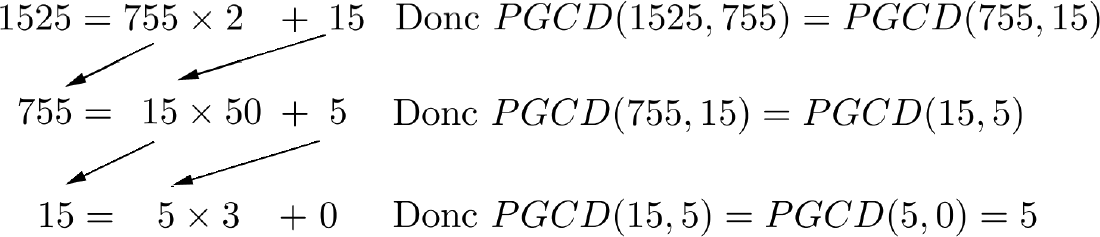
\includegraphics[width=0.7\textwidth]{images/euclide.png}
\end{center}
\end{exemple}

\begin{rem}
\begin{enumerate}
\item Le procédé précédent est un algorithme : <<ensemble de règles opératoires dont l'application permet de résoudre un problème énoncé au moyen d'un nombre fini d'opérations>>.
\item Pour coder des algorithmes nous utiliserons :
\begin{enumerate}
\item des variables (ici $a,b,r$) qui auront des valeurs assignées;
\item des instructions : des affectations, des opérations,...;
\item des expressions logiques : ici dire si le reste est nul ou non;
\item des boucles : (ici une boucle Tant que) pour répéter des instructions;
\item une rédaction sous forme de fonction : pour pouvoir appeler cet algorithme à d'autres endroits de notre programme.
\end{enumerate}
\end{enumerate}
\end{rem}

\begin{minipage}[c]{.48\linewidth}
\begin{py}
Codage en Pythonde l'algorithme d'Euclide :
\begin{python}
def Euclide_PGCD(a,b):	# on définit le nom de la 
			# fonction et ses variables 
			#d'entrées/d'appel
    r=a%b		# on calcule le reste dans 
			# la division de a par b
    
    while r!=0:		# tant que ce reste est non nul :
        a=b		# b devient le nouveau a
        b=r		# r devient le nouveau b
        r=a%b		# on recalcule le reste
        
    return(b)		# une fois la boucle terminée, 
			# on retourne le dernier b    
print(pgcd(1525,755))	# on affiche le résultat 
			# retourné par la fonction
\end{python}
\end{py}
\end{minipage}\hfill
\begin{minipage}[c]{.48\linewidth}
\begin{pseudo}
\begin{tabular}{p{.9\textwidth}}
\hline
Fonction PGCD : algorithme d’Euclide \\
\hline
\textbf{Données :} a et b : deux entiers naturels non nuls tels que a > b \\
\textbf{Résultat :} le PGCD de a et b \\
\\
\textbf{Euclide\_PGCD}(a,b) \\
\hspace{.5cm}\textbf{Répéter}\\
\hspace{1cm}r $\leftarrow$ a mod b\\
\hspace{1cm}a $\leftarrow$ b \\
\hspace{1cm}b $\leftarrow$ r \\
\hspace{.5cm}\textbf{Jusqu’à} r == 0 \\
\hspace{.5cm}\textbf{Retourner} a\\
\hline
\end{tabular}
\end{pseudo}
\end{minipage}

A la nième itération, on a la relation a $a_n=q_n\times b_n +r_n$ où $q_n$ est un entier. 

\subsection{Définitions}
\begin{defi}
\textbf{Variables}

Une variable permet de stocker des informations. Une variable est définie par :
 \begin{multicols}{2}
\begin{itemize}
\item un identificateur (nom de la variable);
\item un type;
\item une valeur;
\item une référence;
\item des opérations. 
\end{itemize}
\end{multicols}
\end{defi}



\begin{defi}
\textbf{Identificateur}

L'identificateur correspond au nom de la variable. Il doit être explicite. Pour nommer une variable, il est possible d'utiliser :
\begin{itemize}
\item les lettres de l'alphabet en minuscules (\textbf{a $\rightarrow$ z}) ou en majuscules (\textbf{A $\rightarrow$ Z}) ;
\item des chiffres (\textbf{0 $\rightarrow$ 10});
\item l'underscore \textbf{\_}.
\end{itemize}

Le nom d'une variable commence par une lettre.

\end{defi}

\begin{rem}
En python, les noms de variables suivants sont interdits : 
\begin{center}
\textsf{
\begin{tabular}{lllllllll}
and & as & assert & break & class & continue & def & True & try \\
del & elif & else & except & False & finally & for & while & \\
from & global & if & import & in & is & lambda & with & \\
None & nonlocal & not & or & pass & raise & return & yield& \\
\end{tabular}}
\end{center}
\end{rem}

\begin{exemple}
\textit{Lister les identificateurs utilisés dans l'algorithme d'Euclide.}
\end{exemple}


\begin{defi}
\textbf{Affectation}

L'affectation permet d'assigner une valeur à une variable.
\end{defi}

\begin{exemple}
\begin{minipage}[c]{.35\linewidth}
\begin{pseudo}
\begin{algorithm}[H]
nbBooleen $\gets$ True\\
nbEntier $\gets$ 2\\
nbReel $\gets$ 3.456\\
chaine $\gets$ "coucou"\\
\end{algorithm}
\end{pseudo}
\end{minipage}\hfill
\begin{minipage}[c]{.3\linewidth}
\begin{py}
\begin{python}
nbBooleen = True
nbEntier = 2
nbReel = 3.456
chaine = "coucou"
\end{python}
\end{py}
\end{minipage}\hfill
\begin{minipage}[c]{.3\linewidth}
\begin{sci}
\begin{scilab}
nbBooleen = %T
nbEntier = 2
nbReel = 3.456
chaine = "coucou"
\end{scilab}
\end{sci}
\end{minipage}
\end{exemple}


\begin{defi}
\textbf{Typage}

Le typage correspond à la nature de la variable (booléen, nombre entier, nombre réel \textit{etc}). 

On parle de typage statique lorsqu'il est nécessaire de définir le type d'une variable lors de sa création. On parle de typage dynamique lorsque, par exemple, le type le mieux adapté est choisi automatiquement lors de l'assignation d'une variable.
\end{defi}

\begin{exemple}
\begin{minipage}[c]{.9\linewidth}
\begin{py}
\begin{python}
# type permet de determiner le type d'une variable
>>> type(nbBooleen)
        <class 'bool'>
\end{python}
\end{py}

\end{minipage}\hfill
\begin{minipage}[c]{.45\linewidth}
\end{minipage}
\end{exemple}

\begin{defi}
\textbf{Référence}

La référence permet de créer un alias pointant directement vers l'adresse mémoire d'une variable.
\end{defi}

\begin{defi}
\textbf{Opérations}

Une opération est une combinaison arithmétique de deux ou plusieurs variables. Le résultat dépend du type de variable. 

Les principales opérations sont les suivantes : 
\begin{multicols}{2}
\begin{itemize}
\item l'addition : \textbf{+};
\item la soustraction : \textbf{-};
\item la multiplication : \textbf{*};
\item l'exposant :\textbf{**};
\item la division : \textbf{/};
\item la division entière : \textbf{//};
\item le modulo : \textbf{\%};
\item la valeur absolue : \textbf{abs}.
\end{itemize}
\end{multicols}
\end{defi}




\subsection{Types de variables}

\subsubsection{Types simples}
\begin{defi}
\begin{itemize}
\item les entiers
\item les réels
\item les booléens
\item les caractères
\end{itemize}
\end{defi}


\begin{exemple}
\begin{minipage}[c]{.45\linewidth}
\begin{py}
\begin{python}
>>> a = 64 # affectation d'un entier
>>> a = 64.64 # affectation d'un reel
>>> a = True # affectation d'un booleen
>>> a = "a" # affectation d'un caractere
\end{python}
\end{py}
\end{minipage}\hfill
\begin{minipage}[c]{.5\linewidth}
\begin{sci}
\begin{scilab}
--> a = 64 // affectation d'une constante
--> a = int8(64) // aff. un entier sur 8 bits
--> a = int16(64) // aff. un entier sur 16 bits
--> a = %T // affectation d'un booleen
--> a = "a" // affectation d'un caractere
\end{scilab}
\end{sci}
\end{minipage}
\end{exemple}

\begin{rem}
En programmation, le type entier (\textsf{int} -- \textsf{integer}) désigne les entiers \textbf{relatifs}.
\end{rem}

\begin{exemple}
Il est aisé de convertir des nombres depuis une base $n$ vers la base décimale : 

\begin{minipage}[c]{.45\linewidth}
\begin{py}
\begin{python}
>>> 0b1000000 # Conv. binaire>decimal
	64
>>> 0x40 # Conv. hexa. > decimal
	64
\end{python}
\end{py}
\end{minipage}\hfill
\begin{minipage}[c]{.45\linewidth}
\end{minipage}
\end{exemple}




\subsubsection{Les chaînes de caractères}
\begin{defi}
Les chaînes de caractères sont une succession de caractères. 
\end{defi}

\begin{rem}
En raison des différences d'encodages entre les différents systèmes d'exploitation, des problèmes peuvent se poser lors de l'affichage des caractères spéciaux tels les accents, les cédilles ...
\end{rem}

\begin{rem}
\textit{Séquences d'échappements}
L'utilisation d'un antislash \\ dans une chaîne de caractère peut entraîner un comportement particulier de cette chaîne de caractère : 
\begin{itemize}
\item \textbf{\textbackslash n} provoque un retour à la ligne (retour chariot);
\item \textbf{\textbackslash t}  provoque une tabulation;
\item \textbf{\textbackslash a} provoque une bip système;
\item \textbf{\textbackslash "} et \textbf{\textbackslash '} permettent d'écrire un guillemet sans ouvrir ou fermer une chaîne de caractère;
\item \textbf{\textbackslash\textbackslash} permet d'écrire un antislash.
\end{itemize}
\end{rem}

\begin{exemple}
\begin{minipage}[c]{.45\linewidth}
\begin{py}
\begin{python}
>>> a = 64 ; b = "Pyrenees Atlantiques"
>>> print(a,": \t",b)
	64 	 Pyrenees Atlantiques
\end{python}
\end{py}
\end{minipage}\hfill
\begin{minipage}[c]{.45\linewidth}
\end{minipage}
\end{exemple}

\subsubsection{Les listes et les tableaux}

\begin{defi}
\textbf{Liste}

Une liste est une collection de plusieurs éléments qui peuvent avoir un type différent. 
\end{defi}

\begin{exemple}

\begin{minipage}[c]{.6\linewidth}
\begin{py}
\begin{python}
>>> x=[1,"b",3,"coucou"] # Creer une liste
>>> print(x[0]) # Acces a une variable
>>> print(x[0:2]) # Acces de x[0] a x[1]
>>> x.append(5) # Ajouter un element en fin de liste
>>> del(x[2]) # Supprime x la valeur 3
\end{python}
\end{py}
\end{minipage}\hfill
\begin{minipage}[c]{.45\linewidth}
\end{minipage}
\end{exemple}
%Listes en intension ? res =[x**2 for x in range (1,10)]

\subsubsection{Les dictionnaires}
\begin{defi}
Les dictionnaires sont des collections de clés auxquelles sont associées des valeurs. 
\end{defi}

\begin{exemple}
\begin{minipage}[c]{.45\linewidth}
\begin{py}
\begin{python}
>>> dep = {"Ain":1}
>>> dep["Aisne"]=2
>>> print(dep)
	{'Aisne': 2, 'Ain': 1}
>>> print(dep['Ain'])
	1
\end{python}
\end{py}
\end{minipage}\hfill
\begin{minipage}[c]{.45\linewidth}
\end{minipage}
\end{exemple}





\section{Expressions et instructions simples}


%Affection simple :
%\begin{itemize}
%\item variable = valeur
%\item Création et mémorisation de l'identificateur de la variable
%\item Attribution d'un type (typage dynamique)
%\item Création et mémorisation de la valeur
%\item Lien entre l'identificateur et l'emplacement mémoire correspondant (référence)
%\end{itemize}



\subsection{Expressions}

\begin{defi}
\textbf{Expression}

Une expression est l'évaluation d'un calcul. Un résultat est retourné. 
\end{defi}

\begin{exemple}
\begin{minipage}[c]{.45\linewidth}
\begin{py}
\begin{python}
>>> 1+1
	2
>>> 'a'+'a'
	'aa'
>>> 1 == 1
	True
\end{python}
\end{py}
\end{minipage}\hfill
\begin{minipage}[c]{.45\linewidth}
\begin{sci}
\begin{scilab}
--> 1+1
	ans = 2
--> 'a'+'a'
	ans = aa
--> 1 == 1
	ans = T
\end{scilab}
\end{sci}
\end{minipage}
\end{exemple}


\subsection{Instructions}


\begin{defi}
\textbf{Instruction}

Une instruction est une action utilisée dans un algorithme ou dans un programme. Une instruction peut inclure une expression.
\end{defi}

\begin{exemple}
\begin{minipage}[c]{.3\linewidth}
\begin{pseudo}
\begin{algorithm}[H]
$a\gets 1$\\
Afficher(a)\\
Type\_De(a)
\end{algorithm}
\end{pseudo}
\end{minipage} \hfill
\begin{minipage}[c]{.3\linewidth} 
\begin{py}
\begin{python}
>>> a = 1
	1
>>> print(a)
	1
>>> type(a)
	<class 'int'>
\end{python}
\end{py}
\end{minipage}\hfill
\begin{minipage}[c]{.3\linewidth}
\begin{sci}
\begin{scilab}
--> a = 1
	ans = 1.
--> mprintf("%f",a)
	1.0000
--> typeof(a)
	ans = constant
\end{scilab}
\end{sci}
\end{minipage}
\end{exemple}



\begin{rem}
En python, les expressions ou les instructions sont séparés par des \textbf{;} ou par des retours à la ligne.
\end{rem}


\subsection{L'affectation}

\subsubsection{L'affectation simple}
On a vu précédemment, qu'il était possible d'affecter assez simplement une valeur à une variable. Lors d'une affectation, 
un espace mémoire est réservé dans la mémoire de l'ordinateur. Cet espace mémoire est situé à une certaine adresse.

À cette variable on fait correspondre un identificateur (nom de la variable), une valeur, un type (booléen, entier, flottant ...) et une adresse mémoire.

\textbf{Tant que la variable n'est pas réaffectée, l'adresse mémoire reste inchangée.}

\begin{rem}
\begin{minipage}[c]{.55\linewidth}
\begin{py}
\begin{python}
>>> a=2
>>> id(a) # Permet de connaitre l'adresse memoire
    15590464
\end{python}
\end{py}
\end{minipage}
\end{rem}




\begin{exemple}

\textit{Affectation simple}

Lorsqu'on copie une variable simple, un nouvel espace mémoire avec une nouvelle adresse est créé. 
\begin{minipage}[c]{.45\linewidth}
\begin{pseudo}
\begin{algorithm}[H]
$a \gets 1$ \\
$b \gets a$ \\
\end{algorithm}
\end{pseudo}
\end{minipage}\hfill
\begin{minipage}[c]{.45\linewidth}
\begin{py}
\begin{python}
>>> a=2
>>> id(a) 
    15590464
\end{python}
\end{py}
\end{minipage}%\hfill
%\begin{minipage}[c]{.3\linewidth}
%\begin{sci}
%\begin{scilab}
%--> a=2
%\end{scilab}
%\end{sci}
%\begin{minipage}[c]{.3\linewidth}
%\end{minipage}

\end{exemple}

\subsubsection{L'affectation multiple}

L'affectation multiple permet l'affectation simultanément plusieurs variables.

\begin{exemple}
\textit{Affectation multiple}


\begin{minipage}[c]{.55\linewidth}
\begin{py}
\begin{python}
>>> a,b=1,2
>>> a
    1
>>> b
    2
\end{python}
\end{py}
\end{minipage}

\end{exemple}


\subsubsection{Problèmes liés à l'affectation de variables composites}

\begin{exemple}
\textit{Copie de variables composites}

Les variables comme les tableaux ne peuvent pas être copiées aussi simplement que les variables simples :


\begin{minipage}[c]{.55\linewidth}
\begin{py}
\begin{python}
>>> a,b=1,2
>>> tab1=[a,b]
>>> tab2=tab1
>>> id(tab1);id(tab2)
    19282320
    19282320
\end{python}
\end{py}
\end{minipage}

Lors de la création de tab2, python n'a pas créé un nouvel espace mémoire. Il a juste créé la variable tab2 et lui a adressé le même espace mémoire que tab1. En conséquence, si on change un champ de tab1, le même champ de tab2 sera modifié. En général, ce comportement n'est pas souhaité:

\begin{minipage}[c]{.55\linewidth}
\begin{py}
\begin{python}
>>> tab1;tab2
    [1, 2]
    [1, 2]
>>> tab1[0]=0
>>> tab1;tab2
    [0, 2]
    [0, 2]
\end{python}
\end{py}
\end{minipage}

Ainsi, pour copier un tableau, une liste ou un dictionnaire, il est nécessaire d'utiliser une méthode spéciale qui permettra de recréer une nouvelle variable avec une nouvelle adresse mémoire.
l
\begin{minipage}[c]{.55\linewidth}
\begin{py}
\begin{python}
>>> tab2=tab1.copy()
>>> id(tab1);id(tab2)
    19282320
    20335832
>>> tab1[0]=4;tab1;tab2
    [4, 2]
    [0, 2]
\end{python}
\end{py}
\end{minipage}\hfill
\begin{minipage}[c]{.3\linewidth}
\end{minipage}

\end{exemple}


\begin{rem}
En Python, le passage des éléments se fait toujours par référence. Il faudra donc prendre garde à la manipulation des variables, notamment lorsqu'on leur applique des fonctions. 
 
\end{rem}

\subsubsection{Affectation externe}

Lors de l'exécution d'un programme, il est possible de demander à l'utilisateur de saisir une donnée. Pour cela il existe des instructions permettant de communiquer avec l'utilisateur.

\begin{exemple}
\begin{minipage}[c]{.45\linewidth}
Dans Python, en utilisant la fonction \textsf{input}, les données saisies par l'utilisateur sont converties en chaîne de caractère.
\begin{py}
\begin{python}
>>>a=input()
\end{python}
\end{py}
\end{minipage}\hfill
\begin{minipage}[c]{.45\linewidth}
\end{minipage}
\begin{sci}
\begin{scilab}
-->a=input("Saisir un nombre : ")
\end{scilab}
\end{sci}
\end{exemple}

\subsection{Sorties à l'écran}
Lors de l'exécution d'un programme il est souvent nécessaire que ce dernier renvoie des informations à l'utilisateur pour, par exemple, donner le résultat d'une opération ou encore donner l'avancement dans le programme.

\begin{exemple}
\begin{minipage}[c]{.95\linewidth}
\begin{py}
\begin{python}
>>> print("Coucou") # Afficher une chaine de caract.
    Coucou
>>> i = 2
>>> print("La valeur de i est '',i,''.'',sep='') # Afficher une phrase composee.
    La valeur de i est 2. # sep='' permet de supprimer l espace entre 2 et le point
\end{python}
\end{py}
\end{minipage}

\begin{minipage}[c]{.95\linewidth}
\begin{sci}
\begin{scilab}
print(%io(2),a)     // affiche le contenu de la variable a a l ecran
write(%io(2),a)    // fonction similaire
disp(a)               // affiche le contenu de a sans faire figurer a = 
xinfo('message')  // affiche un message dans la barre d information
\end{scilab}
\end{sci}

\end{minipage}
\end{exemple}

\subsection{Gestion des exceptions}
%Gestion des exceptions : try, except (python), try, catch (scilab)


Certaines parties de programmes sont susceptibles de produire des erreurs. C'est par exemple le cas d'une entrée-sortie hasardeuse (saisie au clavier, lecture d'un fichier volumineux) ou bien de l'utilisation d'une opération instable dont le résultat peut provoquer un dépassement…
 
Pour gérer cette situation, on peut utiliser une structure : \textsf{try} -- \textsf{except} en Python ou \textsf{try} -- \textsf{catch} avec Scilab.

\textsf{except} permet de spécifier une action de remplacement en cas d'erreur.

\begin{minipage}[c]{.95\linewidth}

\begin{py}
\begin{python}
try :
    nombre = int(input("Sasir un nombre : "))
    print ("Le carré de", nombre, "est égale à", nombre*nombre)
except : 
    print("Vous n'avez pas donné de nombre correct, nous ne pouvons donc pas donner le carré") 
\end{python}
\end{py}
\end{minipage}

\textsf{try} fonctionne toujours avec \textsf{except}.

Ce programme demande donc un nombre et affiche son carré. Mais s'il y a eu une erreur lors de la récupération de ce nombre, il affiche qu'il est impossible de donner le carré.

Une solution plus complète serait de redemander un nombre tant que la valeur saisie n'est pas un nombre. Pour cela on peut implémenter les lignes de code suivantes :
\begin{py}
\begin{python}
nombreIncorrect = True
while nombreIncorrect == True :
    try :
        nombre = int(input("Saisir un nombre : "))
        nombreIncorrect = False
    except :
        print ("Vous n'avez pas donné de nombre correct, nous ne pouvons donc pas donner le carré")
print ("Le carré de", nombre, "est égale à", nombre*nombre)
\end{python}
\end{py}


On crée ici une variable ayant la valeur \textsf{True} pour indiquer que la proposition effectuée est incorrecte. Tant que l'utilisateur ne saisit pas de nombre, nombreIncorrect reste égal à \textsf{True}; on continue donc à demander un nombre et on spécifie l'erreur à l'utilisateur.

Comme on a initialisé la variable à \textsf{True}, on entre dans la boucle. Si l'utilisateur saisi réellement un un nombre, on indique avec \textsf{"nombreIncorrect = False"} que l'on ne doit pas refaire un tour de boucle. La question n'est donc pas reposée. 

On sort donc de la boucle lorsqu'on est sûr que la variable nombre contient un nombre. On peut donc afficher le carré.

On peut aussi utiliser la méthode montrée en exemple dans la documentation de python : 
\begin{py}
\begin{python}
while True :
    try :
        nombre = int(input("Un nombre s'il vous plait : "))
        break
    except :
        print ("Vous n'avez pas donné de nombre correct, nous ne pouvons donc pas donner le carré")
print ("Le carré de", nombre, "est égale à", nombre*nombre)
\end{python}
\end{py}

\textsf{While True :} ne s'arrête jamais, c'est une boucle infinie. On demandera toujours un nombre, sauf si on arrête la boucle avec \textsf{break}. Comme le \textsf{break} est dans le \textsf{try}, la boucle s'arrêtera seulement s'il n'y a pas d'erreur, c'est-à-dire que le nombre n'est pas incorrect.
	
Les exceptions permettent donc de gérer, dans un certaine mesure, les erreurs.

De la même manière, sous scilab :
\begin{sci}
\begin{scilab}
try
	<instructions "normales">
catch
	<instructions executees en cas d'erreur>
end
[message_erreur, numero_erreur] = lasterror(%t) // enregistrement de l erreur
<suite du script>
\end{scilab}
\end{sci}

Scilab exécute le code entre les commandes \textsf{try} et \textsf{catch}; si aucune erreur ne se produit, il va tout de suite après le \textsf{end}.

Si une erreur se produit entre le \textsf{try} et le \textsf{catch}, il exécute directement les instructions entre le \textsf{catch}.



\section{Notions de programmation orientée objets}
%\subsubsection{Définitions}
\begin{defi}
\textbf{Classes, objets et méthodes}
Une classe est une structure particulière de programmation. Par instanciation d'une classe, il est alors possible de créer des objets. 

Une classe définit les attributs et des méthodes qui pourront être appliquées à l'objet.
\end{defi}

\begin{exemple}

Nous allons créé une classe permettant de gérer des points dans $\mathbb{R}^3$.

\begin{minipage}[c]{.9\linewidth}
\begin{py}
\begin{python}
class Point3d(object):
	"""Creation d'un point de l'espace"""

p = Point3d()
\end{python}
\end{py}
\end{minipage}
\end{exemple}

\begin{defi}
Un attribut est une donnée propre à l'objet.
\end{defi}

\begin{exemple}

Le point \texttt{p} a comme attribut ses 3 coordonnées. On pourrait donc créer un point à partir de ses coordonnées.

\begin{minipage}[c]{.9\linewidth}
\begin{py}
\begin{python}
class Point3d(object):
    """ Point de l'espace $\mathbb{R}^3$"""
    def __init__(self,coordx,coordy,coordz):
        """Creer un point a partir de 3 coordonnees x, y et z"""
        self.x = coordx
        self.y = coordy
        self.z = coordz

>>> p = Point3d(1,2,3)
>>> p.x
	3
\end{python}
\end{py}
\end{minipage}
\end{exemple}

\begin{defi}
\textbf{Méthodes}


\end{defi}


\begin{exemple}

Le point \texttt{p} a comme attribut ses 3 coordonnées. On pourrait donc créer un point à partir de ses coordonnées.

\begin{minipage}[c]{.9\linewidth}
\begin{py}
\begin{python}
import math

class Point3d(object):
    """ Creation d'un point de l'espace"""

    def __init__(self,coordx,coordy,coordz):
        """Creer un point a partir de 3 coordonnees x, y et z"""
        self.x = coordx
        self.y = coordy
        self.z = coordz

    def distance(self,pt):
        """ Calcule la distance entre 2 points"""
        dist = math.sqrt((self.x-pt.x)**2
                         +(self.y-pt.y)**2
                         +(self.z-pt.z)**2)
        return dist
    
>>> p1=Point3d(0,0,0)
>>> p2=Point3d(1,1,1)
>>> p1.distance(p2)
	1.7320508075688772
\end{python}
\end{py}
\end{minipage}
\end{exemple}

\begin{thebibliography}{2}
\bibitem{gs}{\textit{Gérard Swinnen}, Apprendre à programmer avec Python 3.}
\bibitem{rc}{\textit{Robert Cordeau}, Introduction à Python 3.}
\bibitem{pb}{\textit{Patrick Beynet}, Cours d'informatique en CPGE, Lycée Rouvière Toulon, UPSTI.}
\bibitem{ap}{\textit{Adrien Petri et Laurent Deschamps}, Cours d'informatique en TSI 1, Lycée Rouvière Toulon.}
\end{thebibliography}
\end{document}
